% !TeX root = ../main.tex

\chapter{图表公式例子}
\label{cha:chapter02}

\section{整数快速卷积实现}

Winograd 卷积的一般过程包括输入变换(input transform),权重变换(weight transform),矩阵乘法(GEMM)以及输出变换(output transform)。
其中权重的变换只用操作一次,便可以在不同的输入复用。一般考虑到运行时效率,权重变换可以在卷积操作实际执行前操作,从而Winograd 卷积的实际执行过程可以概况为
以下步骤:
\begin{enumerate}
  \item 将输入的图像块转换到 Winograd 域
  \item 执行在 Winograd 域中执行变换后的输入和权重的矩阵乘法
  \item 将矩阵乘法的结果转换回空间域
\end{enumerate}

若使用F(m, r)有m个输出的r-tap FIR滤波器,F(m, r) 接收的输入的大小为 ( m + r - 1), 则 Winograd 卷积算法可以表示为

\begin{align}
\label{eq:winograd1d}
  Y = A^T [(Gg) \circ (B^Td)]
\end{align}

在式 \ref{eq:winograd1d} 中,$\circ$ 表示 Hadamard Product.

Winograd 卷积算法中的矩阵乘法量同输入的尺寸一致,即 $F(m, r)$ 的Winograd 卷积,其中需要执行 m + r -1 个乘法。而更高维度的Winograd 算法 $F(mxn, rxs)$,则可以通过
在对应的 维度嵌套一维的卷积算法\ref{eq:winograd1d} $F(m, r)$ 和 $F(n, s)$ 实现。特别是对于卷积网络中,最为广泛使用的方形滤波器,即卷积核的宽高相等,$F(m x m, r x r)$
表示卷积核尺寸为 $r x r$,对应的输出尺寸为 $ m x m$, 二维的 Winograd 算法可以表示为 :

\begin{align}
\label{eq:winograd2d}
  Y = A^T [(GgG^T) \circ (B^TdB)] A
\end{align}

而与之对应的直接卷积方法中对应的矩阵乘法则为 $m^2r^2$ (输出为$m^2$个,每个输出对应着$r^2$个输入,每个输入都要同filter中的对应值做一次乘法),而这里二维场景的
Winograd卷积实现,其中的乘法操作的规模为 $( m + r - 1)^2$。而在卷积算法的实现中,矩阵乘法(GEMM)无疑是最为占据主导的操作,自然也是效率优化的瓶颈。于是,以乘法的
规模作为复杂度的度量,Winograd 卷积相对于直接卷积方法,实现的复杂度简化为

\begin{align}
  \label{eq:winograd_reduction}
  \frac{m^2r^2}{(m+r-1)^2}
\end{align}

因此,对于较为常用的两类Winograd 卷积实现 F(2, 3), F(4, 3),即卷积核大小均为3,输出的尺寸分别为2和4的卷积,理论上分别可以达到2.25 和 4倍的加速。而在实际的实现中,
还需要考虑到对于输入和输出的变换所带来的额外开销,在卷积的规模,特别是矩阵乘法的规模没有达到一定的限度时,Winograd卷积方法不一定能够实现理论的加速值。
尽管使用更大尺度(输出的尺度和卷积尺度)的Winograd 卷积可以实现更大程度的复杂度简化,但同时也受限于变换过程的数值稳定性,更大尺度的 Winograd 卷积一般也
意味着不准确,可能会存在精度的损失。

另外,关于Winograd 卷积中使用的变换矩阵 $G$, $B^T$, $A^T$ 的具体表示的推导可以通过Cook Toom 算法来实现。具体过程可以概述为,使用拉格朗日插值多项式,将相当于卷积
的多项式乘法,转换为多项式在固定数目的插值点处取值的逐元素乘法。 Cook-Toom算法的缺点是,随着变换大小的增加,变换很快变得不稳定。 但是,它们非常适合卷积神经网络中使用的3x3小卷积。

Winograd快速卷积算法的更一般形式是使用中国剩余定理。 Cook Toom 算法只是其中之一。而这一过程的具体不在本文的范畴,有兴趣的可以参考 Fast Algorithm for Convolutional 
Neural Networks 中的补充材料。


快速卷积算法相对于直接卷积和基于GEMM的卷积(比如im2col,im2row等)的实现的主要一大优化目标在于减小运算中乘法的规模,尽管快速卷积方法往往为实现减少乘法的次数而不惜引入
一些额外的加法操作以及对于输入的变换,但在运算中乘法操作达到一定的规模后,乘法数目减少所带来的计算收益是可以超过这些额外的开销的。值得注意的是,快速卷积方法中为减少乘法
操作而不惜引入加法的这一优化手段,并不是因为加法操作会比乘法操作快,这个概念具体到现代的硬件设备上的乘法和加法实现实际上往往是站不住脚的,而实际上在现代硬件设备中
乘法和加法操作往往是可以聚合(fused)在一起的,也就是乘累加(multiply and acculate)操作。从而即使额外引入加法,在仔细设计算法执行后,在具体的硬件实现中,也不会带来
额外的计算开销。另外,通过在算法设计中添加加法来减少乘法,充分利用FMA实现计算加速,需要考虑到计算中的乘法和加法的平衡,加法操作需要同乘法操作匹配,否则,额外的加法会
带来计算负担,甚至会超过乘法减少和FMA换取的计算量的减少值,从而反而使得计算变得更低效。

而另外一方面,作为另外一种更为常用的快速卷积方法实现,快速傅里叶变换(FFT)方法在整体的形式上同Winograd 方法\ref{eq:winograd1d}类似,
其中的变换过程则会对应为FFT和inverse 类似,其中的变换过程则会对应为FFT和inverse
 FFT,即变换矩阵$G$ 和 $B^T$表示FFT,而$A^T$ 则表示inverse FFT。同时,式\ref{eq:winograd1d} 中的也将对应的修改为复数乘法,同实数乘法不同的是,直接的复数乘法需要
 4 次实数乘法来实现。然而,卷积网络中的输入往往都是实数,而实数的傅里叶变换存在Hermitian对称性,从而可以将矩阵复数乘法的复杂度减半,只需计算矩阵中的一半的值,另外一半
 只需要取对应的已计算值的共轭复数即可。但即便如此,FFT卷积实现中仍然需要达到 64x64 的输入尺度才能在乘法规模的优化程度上达到和 Winograd 卷积 F(4, 3) 在输入为6x6 时的
 同等水准,使用FFT实现卷积操作的加速需要相比于Winograd卷积更大的内存需求,

 下面对于卷积实现中的一些符号做如下约定。卷积操作作用于输入特征的局部,并且局部特征的卷积结果输出也仅由这一局部的输入所决定。对于输入局部(input tile)尺寸位 $m x m $,
 卷积核(kernel)尺寸为 $k x k$ ,输出块(output tile)特征大小为 $ r x r $ 的卷积操作,可以记为 $ F(r\times r, k\times k, m\times m) $ .

 \subsection{数据排布}

 卷积网络中常用的数据排布方式(data layout)存在 Channel First 即 NCHW 和 Channel Last 即 NHWC 。而对应的在数据加载的过程中,由于在ARMv8-A 架构下,存在 32 个128位
 SIMD 寄存器,因此每个寄存器可以用来存储 4 个32位整数(int32)或者 16 个8位整数(uint8)或者 8个16位整数(int16)。以32位整数举例,在NCHW 数据排布下,在完成128位的
 数据加载后,一个SIMD 寄存器可以用来储存矩阵中一行的四个值,而在NHWC 数据排布下,同样的单个SIMD寄存器可以用来加载矩阵中位于同一个位置的连续四个通道(channel )的值。
 而在Winograd 快速卷积的实现中,NHWC 的数据表示是具备着实现灵活性上的相当的优势的,特别是在量化计算的场景下,定点(fixed point)表示的数据在计算过程中会频繁涉及数据
 位长(data width)或者说数据精度(precision)的变换,NHWC的表示可以灵活的实现并行算法。同时在考虑不同规模的算法下,NHWC的data layout 也可以实现寄存器的高效利用。
 下面在具体的Winograd 卷积的实现中会做对比和具体的说明。

\section{F(2x2, 3x3, 4x4) 的卷积实现}

\subsection{Winograd变换及逆变换}

Winograd 卷积输入变换最为常用的特征方程是

\begin{align}
  X^T x X = 
  \begin{pmatrix}
    1 & 0 & -1 & 0 \\
    0 & 1 & 1 & 0 \\
    0 & -1 & 1 & 0 \\
    0 & 1 & 0 & -1 \\
  \end{pmatrix}
  x
  \begin{pmatrix}
    1 & 0 & 0 & 0 \\
    0 & 1 & -1 & 1 \\
    -1 & 1 & 1 & 0 \\
    0 & 1 & 0 & -1 \\
  \end{pmatrix}
\end{align}

在这里输入变换的输入特征x 无论是 NHWC 表示还是 NCHW表示,抛开Channel 维度而言,矩阵在平面表示上都是row major 的,即同一行中的元素位于矩阵表示中的更内层。而矩阵x
左乘一个矩阵可以表示为 x 中的行元素的线性组合(这一点会在矩阵乘法一节详细展开说明)。上述矩阵的变换过程可以分为两步:

\begin{itemize}
\item 第一步计算 $X^T x $。这里可以借助矩阵 $X^T$ 的简单形式和矩阵左乘的特性快速实现。
\item 第二部计算 $X^T x X = (X^T(X^T x)^T)$,可见这一计算过程只需将第一步的计算结果转置,再重复第一步的计算过程,最终再将结果转置。
\end{itemize}

在这里简单讨论以下NHWC 表示和NCHW 表示在这里对于这一计算过程的影响。首先使用 NCHW 表示,则一个SIMD 寄存器中将包含处于矩阵中同一行的元素,在实现输入特征同
变换矩阵的乘法中将深度依赖矩阵左乘时,其中行的线性组合性质。同时由于这种数据表示,上述算法中的转置操作也不可避免,而转置操作在硬件实现上则是代价相对较高的一种
操作;更重要的一点是,在量化计算中,NCHW 的表示会为算法设计带来更多的困难,比如这里的输入变换中,如果输入的数据类型是 32 位整数(int32),则在ARMv8-A 中的
SIMD 计算中,可以用 4 个 128位的寄存器来存储一个 4x4 矩阵的值,计算过程和上述的数学表示相差无几。而如果输入的特征是 8 位整数(uint8),则上面的算法就需要重新
设计,或者说,NCHW的数据表示下,不得不针对每种类型的数据重新设计算法。最后,如果考虑到后续的计算,NCHW 表示的计算结果中位于同一寄存器中的值必须分散(scatter)
到不同的位置来实现矩阵乘法,而在NHWC 的布局下,每个寄存器都是同一位置不同channel 的值,对于输入变换过程,可以使用  16个 SIMD 寄存器来表示算法中的 4x4 矩阵,
这一表示允许更加灵活的使用SIMD实现对不同channel 的数据的同步计算,而不必针对于输入数据的位长而重新设计算法,数据位长或者精度只会改变SIMD 计算中可以同时操作
的channel数目,数据位长越低,则能同步处理更多channel的数据,同一个128位的寄存器,可以同时处理4个32位的整数或者8个16位的整数。 

此外,NCHW的data layout 的影响还会受限于变换算法过程中的矩阵大小,$F(3, 2)$ 的情形下矩阵是 4x4 的,而在 $F(3, 4)$ 的场景下,输出的矩阵则是 6x6 的。  如果
使用 NCHW 的表示,这样将会使得寄存器中存储一个6x6 的矩阵变得十分棘手。在32位整数的情形下,需要一个半寄存器来表示6x6矩阵中的一行,这样便只能在算法的过度设计
和寄存器的浪费中二选一了。

在量化计算的场景下,这里输入的特征为被量化后的8位无符号整数,执行16次数据加载之后可以获得 4x4 的输入矩阵,ARMv8-A NEON指令中支持一次加载一个64位寄存器
或者一个128位寄存器,实现中采取一次加载8个8位无符号整数(一个64位寄存器),即这里实际加载到的输入是4x4x8 的。同时在这里考虑到定点计算过程中的溢出的影响
需要将8位整数转换为16位整数,而转换为16位整数之后,同一位置的多个channel的数据刚好占满一个128位的寄存器。最终变换输出的结果也是由16位带符号整数表示。

而对于权重变换而言,在通用的Winograd 卷积变换中,同上述输入变换所对应的权重变换矩阵G 为 
\begin{align}
G = 
\begin{pmatrix}
  1 & 0 \\
  \frac{1}{2} & \frac{1}{2} \\
  \frac{1}{2} & -\frac{1}{2} \\
  0 & 1
\end{pmatrix}
\end{align}

为实现这一计算过程的整数化,只需要对这一矩阵扩大两倍即可,即用于整数计算的权重变换矩阵为

\begin{align}
  \begin{pmatrix}
    2 & 0\\
    1 & 1\\
    1 & -1\\
    0 & 2
  \end{pmatrix}
\end{align}

同时,对应的,由于在权重变换的过程中$G $和$G^T $ 均乘2,所以在最终的输出变换过程中需要对输出值除4。

输出变换矩阵$A^T$ 则仍然使用
\begin{align}
  A^T = 
  \begin{pmatrix}
    1 & 1 & 1 & 0 \\
    0 & 1 & -1 & -1
  \end{pmatrix}
\end{align}

\subsection{数据表示}

讨论数字格式(numerical format)时,有两个主要属性。第一个是动态范围,它是可表示数字的范围。
第二个是动态范围内可以表示多少个值,这又决定了格式的精度/分辨率(两个数字之间的距离)。

对于所有整数格式,动态范围为[-2n-1..2n-1-1],其中n是位数。因此,对于INT8,范围是[−128..127],
对于INT4,范围是[−8..7]。整数型数字可表示值的数量为$2^n$。而32位浮点数的动态范围为$\pm3.4 x 10^38$,
可以表示大约$4.2 x 10^9$的值。 这里可以立即发现FP32更具通用性,因为它能够准确地表示各种分布。
这的确是满足深度学习模型需求的一个属性,在深度学习模型中,权重和激活的分布通常非常不同
(至少在动态范围内)。此外,模型中各层之间的动态范围可能会有所不同。 为了能够用整数格式
表示这些不同的分布,比例因子(scale factor)可以被用于将张量的动态范围映射到整数格式范围
。但是,相比于浮点数,整数可表示值的数量要少得多,即分辨率要低得多。
在很多情况下,比例因子可以是浮点数。因此,即使使用整数,也会保留一些浮点计算。另外一方面,
乘法运算也可以使用位移(shift)实现,这样可以不必乘以scalar factor,从而消除了浮点运算。
在GEMMLWOP中,原本未32位浮点数的比例因子便是使用整数乘法加上移位运算来近似得出的。
在许多情况下,这种近似对精度的影响可以忽略不计。

卷积和完全连接的层涉及将中间结果存储在累加器(accumulators)中。 由于整数格式的动态范围有限,
如果我们将相同的位宽用于权重和激活以及累加器,则可能会很快溢出。 因此,累加器通常以更高的位
宽实现。

两个n位整数相乘的结果最多为2n位数字。 在卷积层中,此类乘法被累加$c·k^2$次,其中c是输入通道的
数量,k是内核宽度(假定为正方形内核)。 因此,为避免溢出,累加器应为$2n + M$位宽,其中M至少
为$\log_2(c⋅k^2)$。 在许多情况下,使用32位累加器,但是对于四位整数及更低版本,可能会使用少于
32位的累加器,具体取决于预期的使用情况和层宽度。

\subsection{矩阵乘法实现}

在输入和权重均经过Winograd 变换之后,变换后的矩阵会执行元素间的乘法,然后将对应位置的乘积结果累加(element-wise addition of Hadamard products)。
表示输出通道为m,输入通道为c的权重值可以在c通道中的所有输入区域被复用,
而 c 通道中位置为 $(i, j)$ 的输入则在所有的$(i,j )$位置输出的区域被复用。 这一观察表明,实际上这一操作本身可以转化为研究较为充分的通用矩阵乘法(GEMM)。
对于输入的channel数为 C,输出的channel数为M,且具有R 个分块的卷积, 在 $F(2, 3)$ 的Winograd 卷积中输入的元素为16个,那么对应的需要执行16 次 $[RxC]x[CxM] $
的矩阵乘法。


\subsubsection{矩阵在内存中的灵活表示}
矩阵在存储空间中是以一整块连续的存储块空间所表示的。在矩阵的存储(storage)中有两个同内存(memory)相关的的关键问题:维度(dimension)和跨度(stride)。

跨度是指在遍历矩阵的过程中,在通过不同维度的过程中需要跨过的字节(bytes)数。跨度的存在可以使得很多矩阵的处理变得更加快速有效,同时,对于跨度的理解也有助于
更加容易的理解矩阵操作的实现。矩阵存储在被成为data buffer 的连续(contiguous)的同质(homogeneous)内存块( block of memory)中。Strides 可以作为一个
矩阵的meta data(元数据)实现多维矩阵之中的不同维度的index(索引)与它在连续memory block中的位置的映射(mapping)。简而言之,strides表示对于每个维度
的连续元素之间的字节间距(byte-separation)。同时矩阵存储空间的同质性也保证了矩阵在存储空间中的连续元素间的单位距离的一致性,比如对于int32类型的矩阵,
这里计量矩阵元素的单位距离就是 4个bytes,每两个矩阵元素在存储中的距离为4。于是对于多维矩阵而言,比如对于int类型的二维矩阵 $A$,$A$ 在矩阵表示的最内侧
的元素在memory中连续存储 ,即二维矩阵中的column(列)元素在实际的存储中相邻,在二维场景下可以成为 row-major。从$A[0, 0]$所表示的元素
移动到$A[0,1]$所表示的元素,即在同一行(第0行)中的元素间,从第0列移动到第1列,这里需要在data buffer中移动4个byte,也就是在列所对应的维度上的一个stride。
然而,如果从$A[0,0]$ 所表示的元素的位置移动到 $A[1, 0]$, 即在同一列(第0列),移动到下一行(从第0行移动到第1行)所在元素的位置,直观而言,需要先遍历
这一行中剩余的元素,才能够到达下一行,然后再下一行中遍历元素到达目标元素,比如矩阵$A$是一个$3x3$大小的矩阵,那么从 $A[0,0]$ 到$A[0,1]$ 需要遍历
$3x4$ 个bytes。也就是说矩阵$A$在行的维度上相邻元素间的间距(row stride)是 12个 bytes。Stride 的存在可以使得矩阵的处理变得更加灵活,也使得很多矩阵操作轻量化,矩阵的转置
以及reshape等操作可以不用实际操作矩阵,而仅仅是改变矩阵各个dimension 所对应的stride这一meta data,比如矩阵的转置实际上可以只是交换对应的stride并且
改变矩阵的shape信息。比如,对于前面例子中的3x3矩阵$A$,假如这里使用$(12, 4)$表示矩阵 $A$在第0维度(row)的stride为 12 个bytes,而在第1维度(column)
的stride为 4个bytes。它的转置$A^T$并不需要对于$A$所对应的内存块中的元素做实际的重新排布 (reorder),而只需要将 $A$原本所对应的stride信息修改为
$(4, 12)$ 即可。同样的,在考虑到矩阵的stride这一元信息(meta info)的场景下,对于举证的处理也不能直观的认为矩阵的最内层(innermost)元素之间的距离
一定是单位该元素数据类型的尺度。而是在沿着矩阵的某个维度实现遍历处理的过程中,这一维度上对应元素间的距离一定是这一维度队对应的stride。

除其他外,基于原有的矩阵的创建一个新的矩阵对象的操作也可以因此而轻量化。创建一个新的数组元数据,该元数据使用相同的data
buffer 来创建该数据缓冲区的新视图,该视图对缓冲区的解释(interpolation)不同(例如,形状,偏移量,字节顺序, 大步等),但共享相同的数据字节。 例如slice 操作,
只需要创建一个新的矩阵元数据信息,对应的更改其起始位置的offset和各个维度的stride,而不需要从memory中拷贝data buffer中的相关数据元素。

\subsubsection{ARMv8-A 架构硬件特征}

ARMv8 指令集架构的设计中包含 32个64位 (doubleword)NEON 寄存器,或者称为 D 寄存器,同时,这32个 D 寄存器也可以视为 16 个 128位(quadword)寄存器,
称为 Q 寄存器。

NEON 作为一个SIMD 并行计算的协处理单元,具有以下流水线执行特征
\begin{itemize}
\item NEON指令运行在其独立的10-stage 的流水线中
\item ARM 在每个执行周期(cycle)可以调度(dispatch)两个NEON 指令
\item 可以容纳16条指令的指令队列(16-entry instruction queue)可以用于在指令实际进入pipeline之前作为缓冲
\item 可以容纳12条数据记录的队列用于存储ARM 寄存器的值,在ARM调度指令之后保存当时ARM 寄存器的值
\end{itemize}

由于以上的特征,在实现ARMv8 指令集的大多架构下,由ARM到NEON(由CPU 处理器到 SIMD 协处理器)的数据传输是相对高效迅速的,而由NEON到ARM 的数据传输则相对
有较高的延时(latency);
同时在ARM 处理器一方不会因为 NEON 协处理器的执行而停滞,除非NEON 协处理器的队列已满。ARM 处理器可以向 NEON 协处理器调度分布一系列的指令后继续处理器
本身的任务,直到NEON 指令的结果返回;
另外,NEON 指令的实际执行同在编写代码中直观观察到的执行并不是一致的,由于队列的存在,NEON 指令的实际执行是有所延后的。这就导致,如果由程序修改了另外一个
程序所需要的缓存行(cache line),会导致ARM 处理器侧的停滞,直到NEON的执行同步。

\subsubsection{硬件相关的矩阵乘法性能优化}
矩阵操作通常是最难实现的,部分原因是潜在解决方案的空间非常之大。 

一个简单的程序,它实际的执行性能起始同硬件架构的环境有着复杂的联系。硬件环境或者程序之中细微的改变可能会对代码的执行效率带来极大的改变。嵌入式场景和
科学计算特别是机器学习领域相关的计算都是需要特别关注代码的执行效率的,因此,必须针对性的对于硬件架构编写高效的程序。尽管实际的硬件环境是及其复杂的,
但在设计硬件相关的高效计算中,仍然存在着相对通用的模型和指导方针。比如提高缓存性能的一大方法,blocking 技术。

定义两个矩阵 $A$, $B$, 对应的尺度分别位 $m x k$, $k x n$, 记为 $A(m, k) $ 和 $ B(k, n) $, 则两者的矩阵乘积可以表示为

\begin{align}
  C(m, n) = A(m, k) x B(k, n)
\end{align}

直观而言,矩阵乘法可以视作是矩阵A 中的行同矩阵 B 中的对应的列的点积的集合,是对应矩阵元素的乘积的和(sum of element-wise multiplication)。简单的伪码
实现如下:

\begin{lstlisting}
\label{code:matmul_naive}
  for (int i = 0; i < m; i++) {
    for (int j = 0; j < n; j++) {
      for (int p = 0; p < k; p++) {
        C(i, j) += A(i, p) * B(p, j);
      }
    }
  }
\end{lstlisting}

对这一简单直接的矩阵乘法的实现的可视化可如下图所示

\begin{figure}
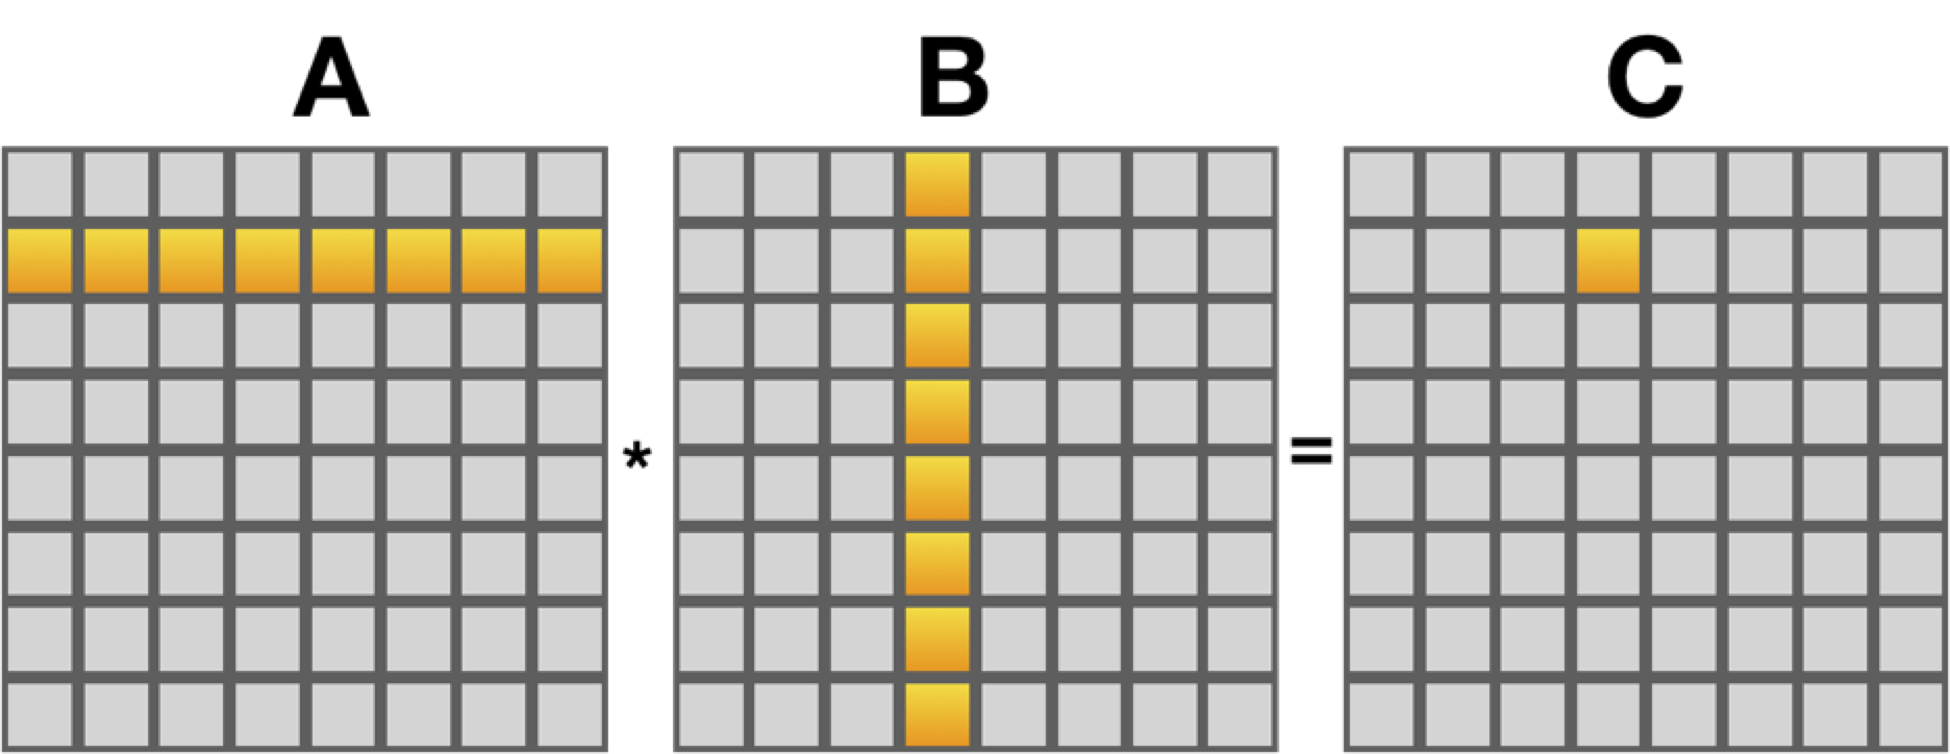
\includegraphics{matmul_naive.png}
\end{figure}

这一矩阵乘法的算法复杂度是$O(n^3)$的。而这一实现实际是非常没有效率的。现代CPU 是普遍具备 SIMD (单指令多数据)支持的,同时在很多的计算指令中,乘法和加法是支持聚合为一个乘累加操作的,即 Multiply and 
Acculturation 或者 FMA(fused multiply-add)。而在方法\ref{code:matmul_naive} 中实现的矩阵乘法实际上是受到内存限制的,从而不能充分利用CPU 的计算能力。而通过SIMD 可以单次处理多个数据的能力,处理器
每次从主内存中(main memory )中加载一个缓存行(cache line )到 L1 高速缓存中,而此后CPU 每次计算则可以从cache line中加载单个数据。尽管这种处理并不理想,但是矩阵B 中处理的情形则更加低效。处理矩阵 B
的过程中,由于矩阵的数据排布(data layout)在这里是 row major 的, 即内存中二维矩阵B 中最内层的储存上相邻的数据实际上是同一行的,的在沿着矩阵的列方向加载 B 中的一个 cache line之后,实际只使用了其中
的一个元素而已,cache line 中包含的是处于同一行的多列元素的值,这些加载到的元素中除了第一个元素被使用到了,其他元素均被浪费。
而在扫描完了B 中整整这一列的数据之后,开始扫描B 的下一列数据时,处理器则早已刷新了缓存。

在矩阵乘法优化中的一种可行的策略是优化 B 中的 memory efficiency,比较直观的一种想法是每次计算中使用从矩阵 B 中加载的 cache line 中的多个元素。将矩阵 A 中的加载的值同矩阵B中加载的多个连续值相乘。而
另外一方面,矩阵乘法有一个属性在于:矩阵 A 乘 矩阵 B 实际上是将矩阵A 中的列以矩阵 B 中的列元素作为参数的线性组合,或者说是,矩阵 B 中的行已矩阵 A 中的行元素作为参数的线性组合。

首先,矩阵的右乘,可以视作列的组合;对于简单的矩阵右乘一个列向量的情形

\begin{equation}
  \begin{pmatrix}
    x_1 & y_1 & z_1\\
    x_2 & y_2 & z_2\\  
    x_3 & y_3 & z_3
  \end{pmatrix}
  \times 
  \begin{pmatrix}
    a \\
    b \\
    c
  \end{pmatrix}
  = 
  \begin{pmatrix}
    ax_1 + by_1 + cz_1\\
    ax_2 + by_2 + cz_2\\  
    ax_3 + by_3 + cz_3
  \end{pmatrix}
\end{equation}

而对于这一过程做一个直观的可视化可以表示为

\begin{figure}
  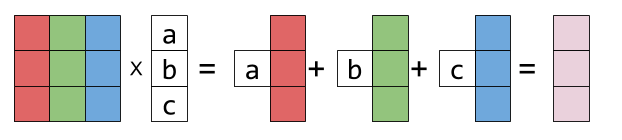
\includegraphics{matvec.png}
\end{figure}

矩阵中的每一列同列向量中的每个元素相乘,矩阵中的一列同列向量中的单个元素(Scalar)的乘积仍是一个列向量,而最终的结果则是这些列向量的和。
这一情形推广到右乘一个矩阵则是相似的情形,乘积的结果的矩阵中的每一列仍是矩阵列的线性组合。

\begin{equation}
  \begin{pmatrix}
    x_1 & y_1 & z_1\\
    x_2 & y_2 & z_2\\  
    x_3 & y_3 & z_3
  \end{pmatrix}
  \times 
  \begin{pmatrix}
    a & d & g\\
    b & e & h\\
    c & f & i
  \end{pmatrix}
  = 
  \begin{pmatrix}
    ax_1 + by_1 + cz_1 & dx_1 + ey_1 + fz_1 & gx_1 + hy_1 + iz_1 \\
    ax_2 + by_2 + cz_2 & dx_2 + ey_2 + fz_2 & gx_2 + hy_2 + iz_2 \\
    ax_3 + by_3 + cz_3 & dx_3 + ey_3 + fz_3 & gx_3 + hy_3 + iz_3
  \end{pmatrix}
\end{equation}

这一过程的可视化表示如下图所示

\begin{figure}
  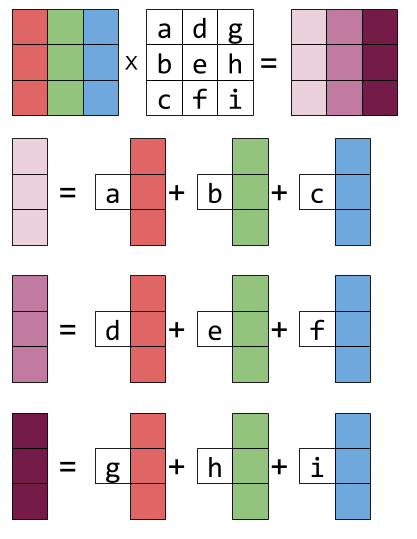
\includegraphics{matmul_right.png}
\end{figure}

而对于左乘一个矩阵则可以视为是矩阵行的线性组合。首先对于一个矩阵左乘一个行向量的情形,可以表示为

\begin{equation}
  \begin{pmatrix}
    a & b & c
  \end{pmatrix}
  \times
  \begin{pmatrix}
    x_1 & y_1 & z_1 \\
    x_2 & y_2 & z_2 \\
    x_3 & y_3 & z_3 
  \end{pmatrix}
  = 
  \begin{pmatrix}
    ax_1 + bx_2 + cx_3 & ay_1 + by_2 + cy_3 & az_1 + bz_2 + cz_3
  \end{pmatrix}
\end{equation}
可视化表示为

\begin{figure}
  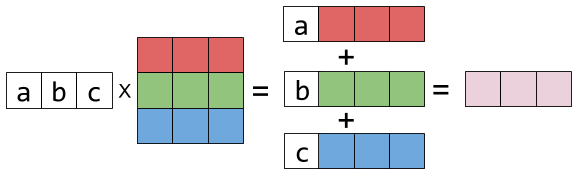
\includegraphics{vecmat.png}
\end{figure}

而在左乘一个矩阵的过程中,则是左乘行向量的情形重复作用于矩阵中的每一行。相对应的可视化表示可以为

\begin{figure}
  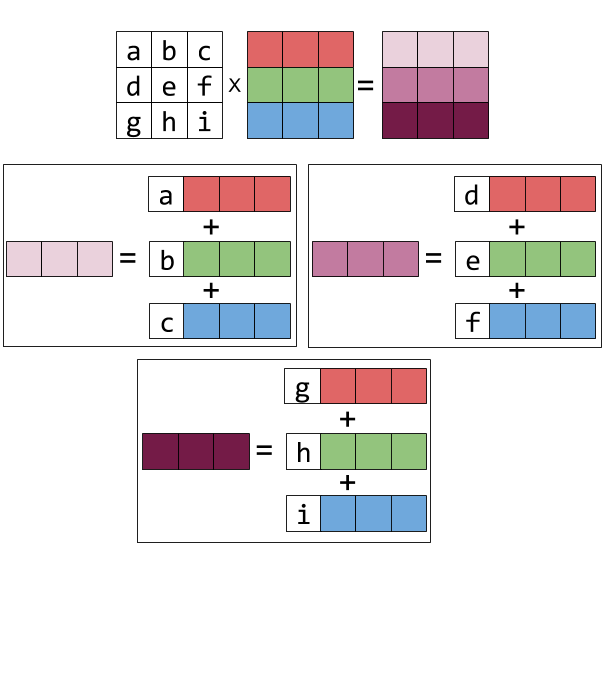
\includegraphics{matmul_left.png}
\end{figure}

于是考虑到矩阵B 的缓存性能的优化策略在于,可以从矩阵A中加载一个元素,并将其广播填满SIMD 寄存器,而矩阵B 中的连续元素也被加载到对应的
SIMD 寄存器,因此两者可以实现元素间乘法的矢量计算,实际上,很多硬件的指令中是支持按照矢量寄存器的 data lane 进行计算的,完全可以
加载A 中的多个元素到矢量寄存器 R,再以R 中的data lane 实现A中的单个值(Scalar)同B 中加载的多个元素的乘法,而将
单个元素广播填满单个SIMD 矢量寄存器的操作,在存在这一支持的情况下大可不必,同时很可以实现寄存器的节约和运算成本的降低。

这一优化策略使得参与计算的矩阵B 的存储带宽(memory bandwidth)获得了较为充分的利用,而换个角度来看硬件资源的利用,现代CPU 一般存在
多个用于调度分配SIMD 计算的执行端口,和多个用于调度数据存取的端口。这意味着,在一个时钟周期里可以实现调度执行多条读取数据的指令,或者
调度执行多条乘法计算指令。在硬件水平上,处理器中的寄存器间的操作的速度是远远高于缓存的读写性能,而缓存的读写性能又远远高于内存,内存的
读写性能则又远远高于硬盘等外部存储,高性能计计算的过程中对于存储性能的优化的目标在于尽可能的减小访问存储的操作同计算操作的比例,提高
高速设备中数据的利用率,在算法的设计上保证加载到高速设备上的数据得到充分利用,并可复用。而在实现矩阵乘法的背景下,这就意味着,从矩阵 A 中
加载的数据需要被用来执行多次计算操作,这一点可以由上述方法中,A 中的元素同来自B 中的同一 cache line 中不同列的元素做计算而保证;同时,
B 中的元素也需要被用于执行不止一次计算,而要实现这一点,则可以通过加载数据时,从矩阵 A 中每次加载多行的元素,从而使得B 中的每一列的元素
可以得到复用。而从计算结果来看,乘积矩阵 C 中的每一行的元素都是一个矢量累加值,每次处理多行A 中的元素的效应则是,矩阵 C 中处理中需要多个
寄存器来存储这些矢量累加值,从使用一个寄存器到使用一块(patch/block)寄存器因此这一过程。因此,这一过程被称为寄存器 blocking (register blocking)

\begin{figure}
  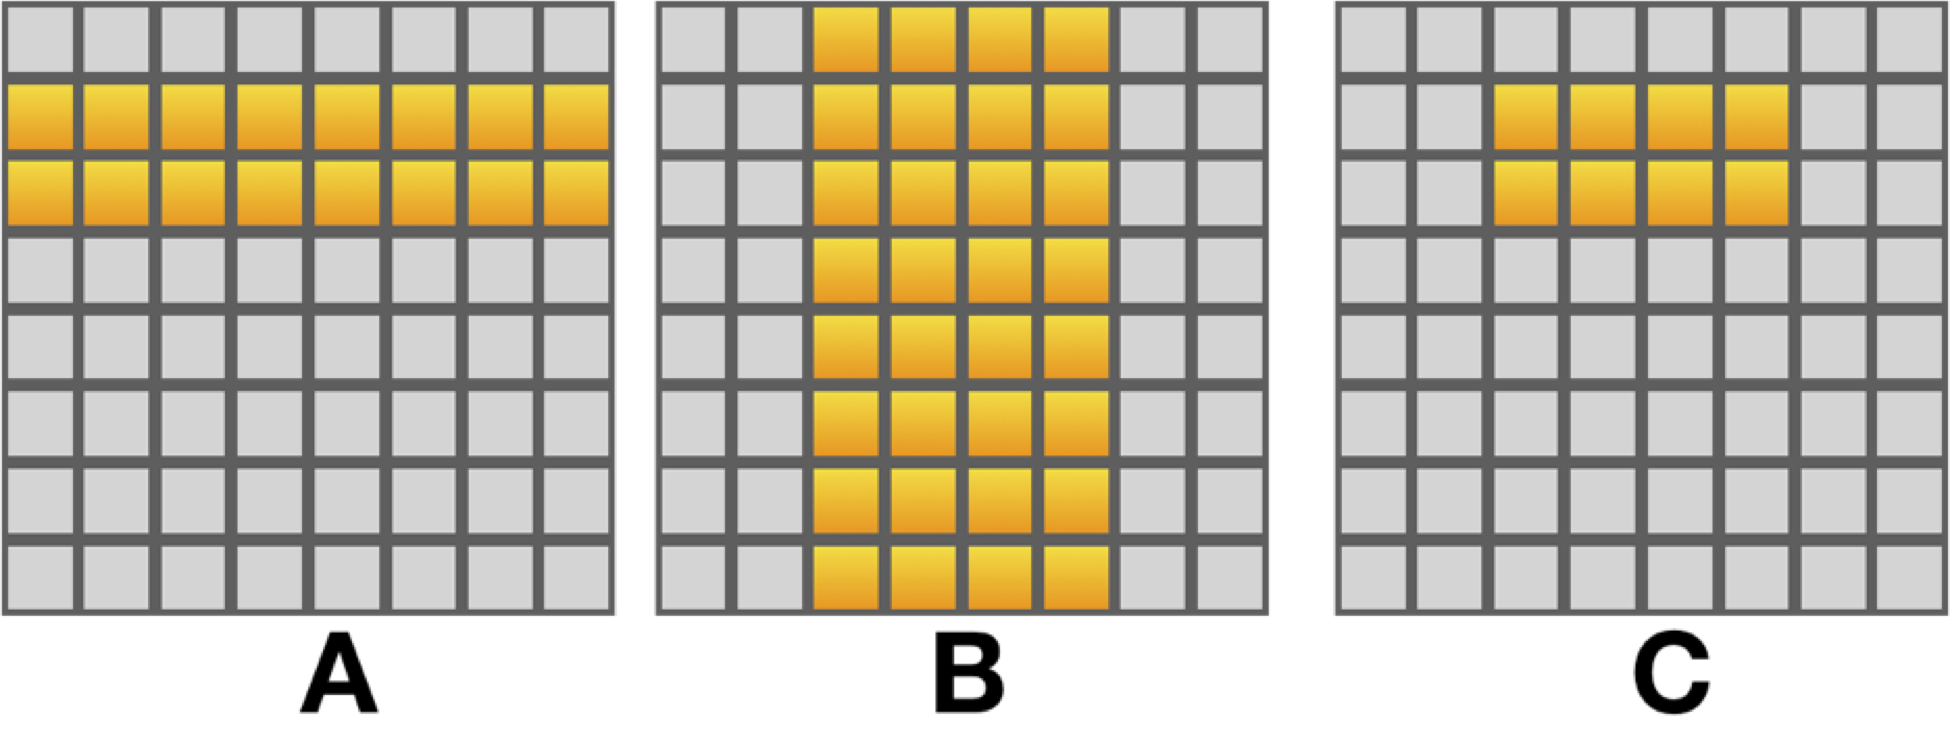
\includegraphics{zregblock.png}
\end{figure}

尽管上述的实现已经让计算中的内存访问机制(memory access pattern)变得相对有效,但是仍然具有着优化的空间。在顺序计算矩阵 C 中的一行中连续
的元素时,需要多次访问呢矩阵 B,加载矩阵B 中不同行的元素,而这一过程中,B 中的值会同时加载到缓存中,由于用于计算的寄存器和缓存都是有限的,
而且一般容量都很小, 这意味着按照这样的顺序访问 B 矩阵,必然 会使得B 的缓存失效。

计算矩阵C 中的一个子矩阵的顺序会影响到矩阵A 和矩阵 B 的内存访问模式。理想的内存访问模式是 将矩阵B加载到我们的L1缓存中,并保存很长时间 。
实现此目的的一种方法是对矩阵C的计算进行分块。而在每次计算中只需要计算 C 中被分割出的这一块即可。对应的伪码实现如下:

\begin{lstlisting}
  \label{code:tiled_matmul}
  for i = 1 to N
    for j = 1 to N
      { read block C{i,j} to fast memory }
      for k = 1 to N
        {read block A{i, k} to fast memory}
        {read block B{k, j} to fast memory}
        
        C{i, j} = A{i, k} * B{k, j} // matrix multiplication on tile
      { write C{i, j} to slow memory }
\end{lstlisting}

假设A, B, C 矩阵都是 $n x n$ 的矩阵,这里对于矩阵的分块每一个小块的尺度则是 $b x b$,记 $N = n / b$ , 这一算法在低速存储设备上的存储访问操作(memory operation)
为

\begin{align}
  NUMBER_MEM_OPS = N \times n^2 // read each block of B N^3 times (N^3 \times \frac{n}{N} \times \frac{n}{N} )
                 + N \times n^2 // read each block of A N^3
                 + 2 \times n^2 // read and write of block C
                 = (2\times N + 2)n^2
\end{align}

于是在这一算法实现下的矩阵乘法中,计算操作同访存操作的比值为 $2\times N^3 / ((2\times N + 2)n^2) \approx n / N = b$,
在 n 足够大是,这一近似成立。因而可以通过矩阵分块计算中的block size块大小实现这一算法的效率提升,同时block size也并不是可以任意大,
这一优化的出发点在于优化利用快速缓存,而这一值同时也受到缓存大小的限制,上述矩阵乘法中的三个块 $A{i, k}, B{k, j}, C{i, j} $ 均必须
不能溢出快速缓存的容量限制,

总结而言,充分考虑到硬件环境的高效矩阵乘法的实现如图所示:

在如下图所示的矩阵乘法算法中。首先,将大小为m,n和k的矩阵乘法在 k 所表示的维度以$k_c$ 大小的高速缓存块进行分割,从而创建rank为k的子问题。 在这一阶段,
为了实现在计算的最基础层次上上,参与计算的元素在存储中是完全连续的,即矩阵表示中最低维度对应的stride为unit stride,需要将B以一种特殊的格式分块打包到连续存储中
(标记为B )。 然后,将每个rank为k的子问题沿m维度,按照缓存块大小$m_c$分块,从而创建block-panel子问题。 然后将当前的$m_c×k_c$块, 记为$A_i$, 按照计算中的
最基础级别,参与计算的元素在存储中是连续的的原则,打包到A。 然后将剩下的该block-panel子问题($C_i:= C_i + A_i B$)实现为高度优化的汇编
计算内核。 而该内核将继续沿$n$,$m_c$划分矩阵,最后在$k_c$维划分矩阵。

\begin{figure}
  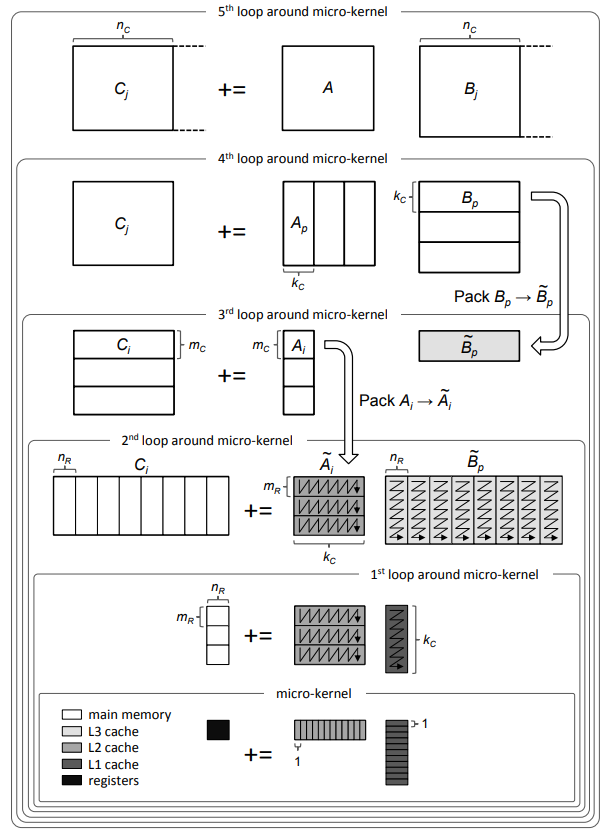
\includegraphics{gemm.png}
\end{figure}

这一矩阵乘法中的多个循环的使用在于根据缓存块大小和寄存器的容量,精心设计矩阵的分块策略,从而使得子矩阵的分布同存储的层级结构相匹配,以达到数据复用的目的。
同时A 和B 的子矩阵被复制打包到临时工作区(workspace),从而使得矩阵乘法操作的micro-kernel能够在内存中连续访问矩阵元素,从而提高了缓存和TLB性能。而一般
打包过程的成本可以通过计算本身来摊销,在计算的规模足够大时,这一成本是可以忽略不记的。

而这其中决定最内层的循环的调用的寄存器相关的参数 $m_r$, $n_r$, 以及较外层的循环调用的高速缓存相关参数 $m_c$, $k_c$, $n_c$ 一般由具体硬件的特性所决定,
比如矢量寄存器的大小,缓存大小,缓存的相关性等。Analytical Modeling Is Enough for High-Performance BLIS 为这些参数的选择提供了一种分析性模型。

\subsection{图片分块方法实现}
在信号处理中,在很多场景下,需要处理的信号都非常长,计算过程中往往没有足够的内存可以容纳需要处理的整段输入。而另外一方面,由于卷积本身是
线性的,因此可以通过简单的将输入的每个输出块相加来计算长序列信号的输出。因此可以通过 overlap-add方法实现长序列的分割,从而将长序列分解成为更易于处理的段序列。
而对于卷积网络中所使用的对于filter 尺寸为 r 且输出为 m 的卷积,通过OLA(overlap-add)方法,卷积的输入被分割为 $m + r - 1$的小块,而块之间存在着 $r-1$ 的重叠(overlap)。而对于
所有输入图像中相同位置的图块,计算输出图像大小为m的图块


\subsection{卷积实现流程概述}

输入的图像或者3D 的特征首先会在空间维度分区,按照上面所述的图片分块方法,分割为$(m+r-1)$ 尺度的小块,记这里
输入的通道数为 C,则每个小块的尺度为 $ (m+r-1) x (m+r-1) x C $。记这里被分割出的小块的数目为 R,这 R 个小块
可以并行的实现到Winograd 域的输入变换,在这一变换过程中 channel维度的变换也是各channel之间相互独立的,因此
这里的输入变换也是通过SIMD 同步在对应的channel实现的。而在变换结束之后,每个输入的小块被转换为Winograd域中的
一个 $ 4 x 4 x C $ 的矩阵,而这样的小块则一共存在R个。而对应于卷积中后续的步骤,这里单个channel中的
4x4 的值需要执行同来自权重变换的 一个channel中的4x4 的权重值的乘法,而变换过程中的指令并行化是在channel维度
实现的,也就是说,在执行一次变换之后,有 4x4 的矢量寄存器,并且每个矢量寄存器中包含有对应位置的连续channel中的
值,这 4x4 个数值需要分发到16 个GEMM 操作,而这里变换之后的输出的值也按照在channel维度连续的方式做储存。即这里
做了输入变换之后的整个特征在内存中的数据排布方式为 16 x R x C. 

在权重的变换方面,要保证输出的channel 的维度在数据的排布方式中位于最内层,即输出通道维度对应的stride 为1。这里同
一般的卷积网络中的数据表示有着相当的不一致,而好在权重的值在做inference的过程中是固定不变的,所以可以预先对权重的
数值做矩阵转置,以保证输出通道在data layout的最内存(实际上权重变换的整个过程都可以在网络运行workload之前完成, 模型运行
中只要复用这个变换值即可)。假如一个 3x3卷积的输入 channel 数为C,而输出的channel 数为 M,每个3x3的权重变换之后为4x4的矩阵,
在channel维度使用矢量计算指令同步计算出权重变换的结果,并将其按照 $ 16 x C x M $ 的layout 写入存储。而在上述的
两种变换过程中,由于寄存器数目有限,并不能一次性处理全部的通道或者特征分块,每次在一部分子块的变换之后将变换结果按照
上述的layout 约束写出的时候,前面所提到的矩阵 stride 的概念便可以使得这一过程实现的非常直观。举个例子来说,输入
变换中处理的第r个子块4x4xC个值可以按照下述方法写出:

\begin{lstlisting}
\label{prog:store}
output := output base address
output += tile_stride
V[4][4] := transformed input
for (i = 0, n = 0; i < 4; i++)
  for (j = 0; j < 4; j++, n++)
    store(output + n* matrix_stride, V[i][j] )
\end{lstlisting}

上述的两者的变换为有效实现矩阵乘法提供了必要的条件。变换后的平面尺度为4x4,所以这里需要16个GEMM计算来实现Winograd域
的乘法操作,而每个GEMM实现中对应的矩阵乘法为一个R x C 的矩阵与C x M 的矩阵的乘积,而前面在变换过程中对于输出的layout
的限制,也是为了在这里可以更方便的实现这些GEMM 计算。当然在实际的卷积计算中R,C,M都可能是比较大的值,这里便需要
精心的设计矩阵乘法,充分利用cache 和 vector register,实现高效计算。毕竟,对于乘法操作的减少是Winograd卷积的最大优势,
高效的GEMM实现才能将Winograd卷积的加速效果真正表现出来,同时,从另外一个角度来看,如果对于Winograd卷积中各个阶段(
输入输出变换,GEMM)的时间占比做一个拆分,在保证GEMM高效实现的前提下,GEMM所占的比重越大,证明Winograd卷积省去的乘法
操作越多,实现的加速效果 越明显。

GEMM执行结束之后,将计算结果按照16xRxM 的layout写出。

类比如输入变换,输出变换的过程可以看作是输入的逆过程,这里将参与输出变换的4x4 多channel 的中间结果从GEMM计算结果的
输出中的16个位置读入,然后通过矢量计算同步处理每个4x4 矩阵多个channel的结果,同时按照对应子块的索引和卷积输出的尺度信息
将输出变换的结果填充到卷积输出的对应位置,从而得到 H x W x M 的卷积输出,完成整个卷积操作。

\begin{figure}
\label{fig:winograd_full_procedure}
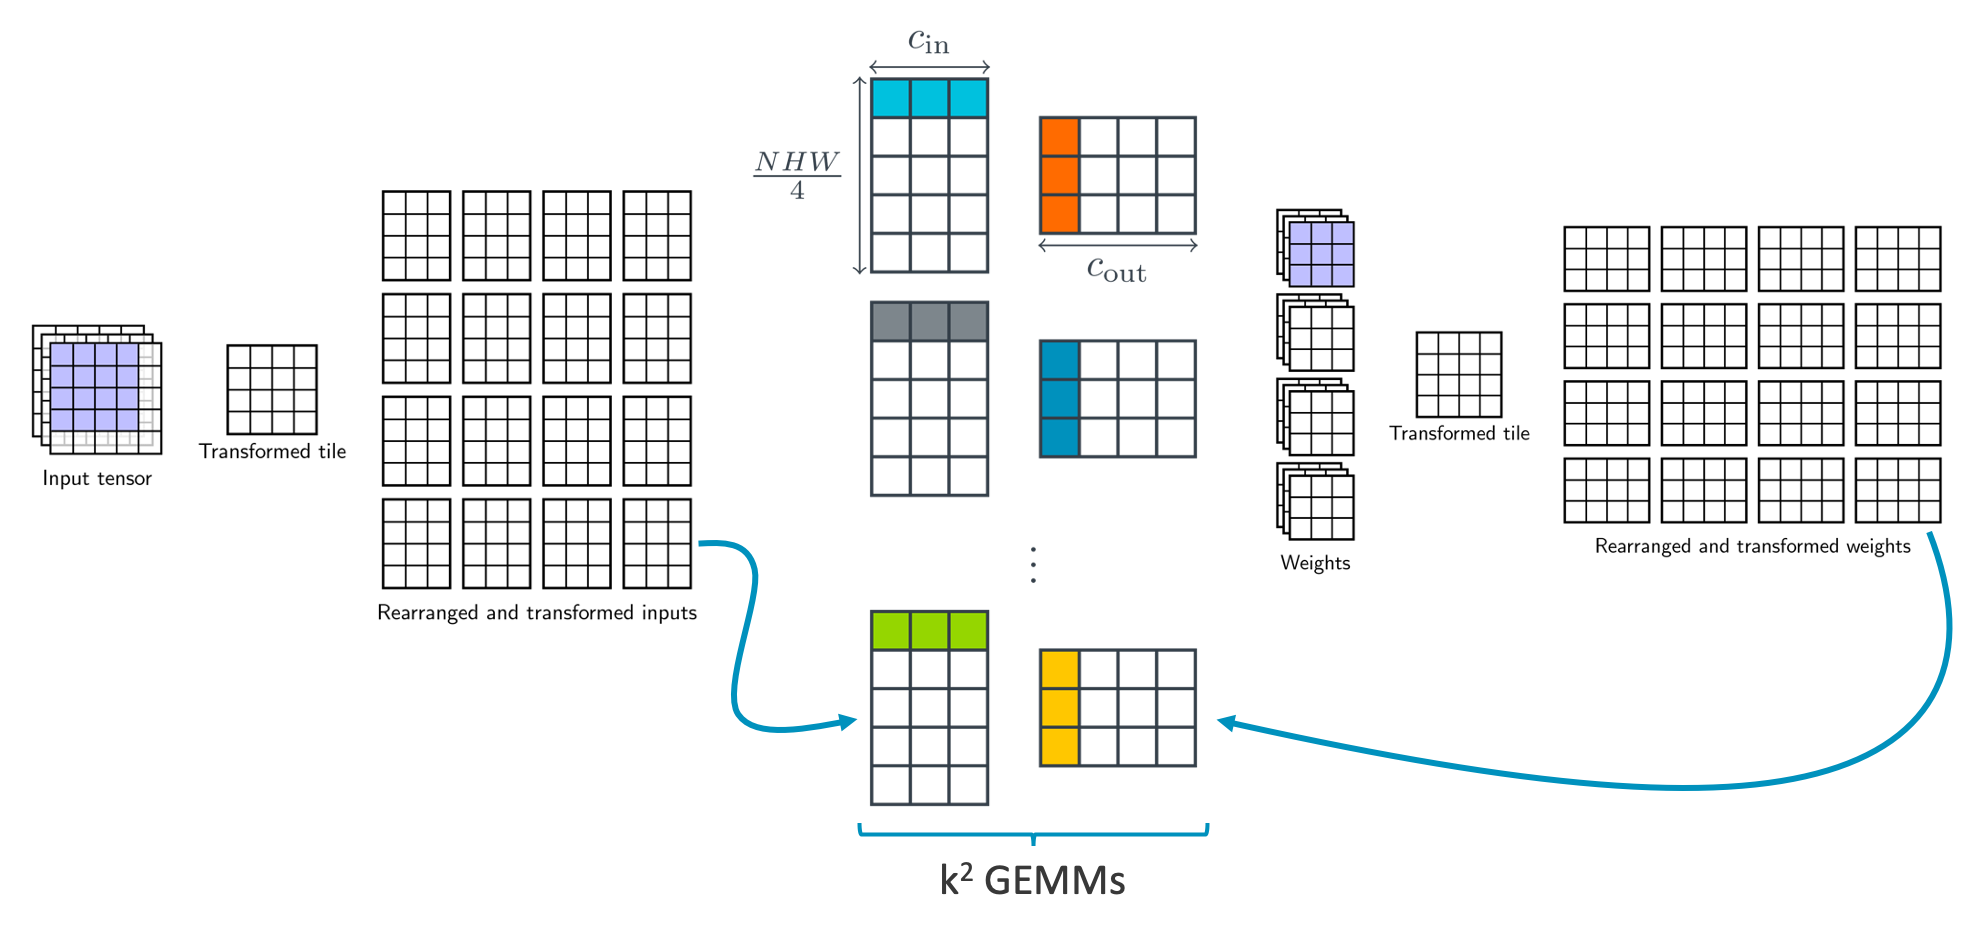
\includegraphics{winograd_conv_process}
\end{figure}

\section{FFT 卷积实现同Winograd 卷积的对比}


\subsection{FFT卷积与Winograd卷积}
离散傅里叶变换方法的有效卷积可以视作 Winograd 卷积 \ref{eq:winograd1d} 的一种特殊情形,其中的矩阵$A^T$, $B^T$ 和 $G$ 均处于复数域,并且由多项式点
( polynomial point)为单位根的范德蒙矩阵(Vandermonde matrices)推导出。

Winograd 与 FFT 卷积中主要能够降低计算成本的一点在于,权重的变换可以预先计算,而卷积输入的变换则可以多次复用,而计算本身中比重最大的部分仍然是矩阵乘法



\iffalse
\section{F(4x4, 3x3, 6x6) 的实现}

最为常用的 F(4, 3) Winograd 卷积中的权重变换矩阵为

\begin{align}
\label{eq:winograd_f43}
  G = 
  \begin{pmatrix}
    \frac{1}{4} & 0 & 0 \\
    -\frac{1}{6} & -\frac{1}{6} & -\frac{1}{6} \\
    -\frac{1}{6} & \frac{1}{6} & -\frac{1}{6} \\
    \frac{1}{24} & \frac{1}{12} & \frac{1}{6} \\
    \frac{1}{24} & -\frac{1}{12} & \frac{1}{6} \\
    0 & 0 & 1
  \end{pmatrix}
\end{align}

将这个变换矩阵转变为整数矩阵需要对其乘24,而对于变换矩阵扩大24倍,将会对于计算带来相当的额外开销。
在执行Winograd 变换时,空间域的权重需要至少额外增加 $floor(\log_{2}{24^2}) = 10$ 位来表示其数值
以免数值溢出。此时如果输入的权重类型为8 位整数,则经过Winograd 变换之后,其数值表示则不得不由32位
整数作表示。而更大位长的数据表示则使得量化计算的效率大幅下降,量化参数的计算或者说定点数据(fixed 
point)的计算,的确在ARMv8-A 架构下会比同样位长的浮点数(floating point)计算更加高效,但这也是在
两者的数据位长相同的情形下,即 int32 的数据计算会比 float32 的计算高效,而如果整数运算需要更长的数据
表示,则整数计算在大多情况下会需要比同它数据表示位长更短的浮点计算效率低。这也就要求在实现量化计算的
过程中,使用整数运算实现原有的算法时,不仅要适度的对参与计算的数据类型作以调整,使用更高精度的数据表示
存储计算的结果,以避免计算的溢出,另外一方面,同时也要保证数据的表示不可以超过浮点运算中最为常用的
数据表示位长,即32位。否则,计算过程的吞吐量则会低于作为对照的浮点运算,这也是违背量化方法实现计算
加速的初衷的。

因此,在这里考虑到数据精度的表示对于计算效率的影响下,这一最为常用的 $F(4, 3)$ Winograd卷积算法
是不可以应用于整数实现的Winograd 卷积计算的。Winograd卷积算法的具体形式的导出,往往是限制在有理数
范围的,这也使得Winograd 卷积算法同FFT 卷积算法相比省去了复数乘法带来的额外开销。然而在有理数域的
数值计算特性也使得常用的Winograd卷积算法在整数计算场景只限于应用于加速效果相对有限的 $F(2, 3)$ 卷积。

而如果考虑到Winograd变换在复数域中可能的取值,则这一问题存在着相对较为简单的表示。尽管在复数域导出
Winograd 算法的动机看似是有点不合理的,毕竟在前文中也提到了Winograd 卷积同基于DFT 的卷积实现的联系,
以及Winograd 卷积相对DFT卷积的优势。Winograd 卷积从效果上来看,可以看作全实数表示的DFT卷积,Winograd
卷积在卷积尺度较小的场景下相对于DFT卷积的优势也正是来自于实数乘法的复杂度低于复数乘法。因此,在Winograd
算法中引入复数,看上去是一个在效率上有所倒退的举动。但实际上,这里的出发点在于获得更加简单的变换矩阵
表示,从而在引入可接受的运算开销的前提下实现量化计算。

最为常用的Winograd $F(4, 3)$ 卷积的形式\ref{eq:winograd_f43}是由 $ [0, 1, -1, 2, -1]$ 五个插值点导出的,
而如果使用对称且相对简单的复数插值点 $[0, 1, -1, i, -i]$,则会导出如下所示的实现F(4,3) 的变换矩阵。

\begin{align}
  B^T = 
  \begin{pmatrix}
    1 & 0 & 0 & 0 -1 & 0 \\
    0 & 1 & 1 & 1 & 1 & 0\\
    0 & -1 & 1 & -1 & 1 & 0 \\
    0 & -i & -1 & i & 1 & 0 \\
    0 & i & -1 & -i & 1 & 0 \\
    0 & -1 & 0 & 0 & 0 & 1
  \end{pmatrix}
\end{align}

\begin{align}
G = 
\begin{pmatrix}
  1 & 0 & 0 \\
  \frac{1}{4} & \frac{1}{4} & \frac{1}{4} \\
  \frac{1}{4} & -\frac{1}{4} & \frac{1}{4} \\
  \frac{1}{4} & \frac{i}{4} & -\frac{1}{4} \\
  \frac{1}{4} & -\frac{i}{4} & -\frac{1}{4} \\
  0 & 0 & 1 \\
\end{pmatrix}
\end{align}

\begin{align}
  A^T = 
  \begin{pmatrix}
    1 & 1 & 1 & 1 &1 &0\\ 
    0 & 1 & −1 & i & −i & 0\\
    0 & 1 & 1 & −1 & −1 & 0\\
    0 & 1 & −1 & −i & i & 1
  \end{pmatrix}
\end{align}

这里导出的变换矩阵使得参与计算的数值的尺度大幅下降,其中输入变换$B^T$ 和 输出变换 $A^T$中均只存在复数加减法,
而权重变换$G$中,数值中最大的分母也由24 减小为4。因此,权重变换在转化为整数运算的过程中,也只需要在原本的数据
表示上乘 $4^2$,而所需的额外的数据表示的位长则为 $\log_{2}(4^2) = 4$ 位。所以,在输入的权重的数据类型位8位整数
的场景下,仍然可以使用 16 位整数表示变换后的结果,而在计算最为密集的矩阵乘法部分也可以实现16位整数的矩阵乘法,
保证这一计算瓶颈的高吞吐。

以下将展开在这一变换表示下的计算复杂度相对于基于GEMM方法的卷积算法的优化。

由于这一方法所导出的各个变换矩阵所有的相似性,这里以输入变换为例说明,其他变换过程均与此过程类似。

\begin{align}
  B^T = 
  \begin{pmatrix}
    1 & 0 & 0 & 0 -1 & 0 \\
    0 & 1 & 1 & 1 & 1 & 0\\
    0 & -1 & 1 & -1 & 1 & 0 \\
    0 & -i & -1 & i & 1 & 0 \\
    0 & i & -1 & -i & 1 & 0 \\
    0 & -1 & 0 & 0 & 0 & 1
  \end{pmatrix}
\end{align}

在上面的变换矩阵中的参数的特殊形式以及矩阵乘法的线性可组合性可知,在输入变换$ B^TdB$ 的计算过程中,第一步计算
$B^Td $ 的结果,对应的第五行和第四行是一对共轭复数。或者这里更加直观的将$B^T d$ 的结果展开:

\begin{align}
  d^*[0, j] = d_{0, j} + d_{4, j}
  d^*[1, j] = d_{1, j} + d_{2, j} + d_{3, j} + d_{4, j}
  d^*[2, j] = -d_{1, j} + d_{2, j} - d_{3, j} + d_{4, j}
  d^*[3, j] = -d_{2, j} + d_{4, j} - i(d_{1, j} - d_{3, j})
  d^*[4, j] = -d_{2, j} + d_{4, j} + i(d_{1, j} - d_{3, j})
  d^*[5, j] = -d_{1, j} + d_{5, j}
\end{align}

而更进一步的,按照前面所述的计算这一变换的实现 $D = B^TdB = (B^T(B^T d)^T)^T$,对上述计算结果转置之后再做同样
的处理之后再做转置,可知变换之后的矩阵,其第四行与第五行的元素,第四列与第五列的元素,分别对应的构成共轭复数。

\fi